\section{Prediction Aggregation}

\begin{table}
  
  \centering
  \tiny
  (a) RMSE values for the five disjoint subsets:

  \vspace{0.4em}

  \begin{tabular*}{0.9\textwidth}{ l l l l l l l }
    \hline
    { } & method & $d_1$ & $d_2$ & $d_3$ & $d_4$ & $d_5$ \\ 
    \hline
    S & svd1          & 1.2389	  & 1.1260	  & 1.1327	  & 1.1045	  & 1.1184	 \\
    S & svd2          & 1.2630	  & 1.1416    & 1.1260	  & 1.1458	  & 1.1260	 \\
    S & svd3          & 1.0061	  & 0.9825	  & 0.9830	  & 0.9815	  & 0.9797	 \\
    S & svd4          & 1.0040	  & 0.9830	  & 0.9849	  & 0.9850	  & 0.9798	 \\
    S & slope\_one    & 1.1919	  & 1.0540	  & 1.0476	  & 1.0454	  & 1.0393   \\
    S & item\_avg     & 1.0713	  & 0.9692	  & 0.9662	  & 0.9683	  & 0.9725	 \\
    S & baseline       & 1.0698	  & 0.9557	  & 0.9527	  & 0.9415	  & 0.9492	 \\
    S & cosine   	    & 1.1101	  & 0.9463	  & 0.9412	  & 0.9413	  & 0.9382	 \\
    S & knn       	  & 1.4850	  & 1.1435	  & 1.1872    & 1.2156	  & 1.2022	 \\
    \hline                                                                    
    A & median    	  & 0.9869	  & 0.8886	  & 0.8857    & 0.8857	  & 0.8855	 \\
    A & average    	  & 0.9900	  & 0.8536	  & 0.8525	  & 0.8525	  & 0.8519	 \\
    A & adaptive       & \textbf{0.9324}	  & \textbf{0.8015}	  & \textbf{0.7993}  & \textbf{0.8238} & \textbf{0.8192} \\
    \hline
  \end{tabular*}

  \vspace{1em}
  
  (b) Statistics for the methods:

  \vspace{0.4em}

  \begin{tabular*}{0.9\textwidth}{ l p{1.8cm} l l l l l }
    \hline
    { } & method & min & max & mean & $\sigma$ & $\Delta$ \\
    \hline
    S & knn       	  & 1.1435	& 1.4850	& 1.2467	& 0.3487 & - \\
    S & svd2          & 1.1260	& 1.2630	& 1.1605	& 0.2277 & 6.9\% \\
    S & svd1          & 1.1045	& 1.2389	& 1.1441	& 0.2197 & 1.4\% \\
    S & slope\_one    & 1.0393	& 1.1919	& 1.0756	& 0.2415 & 5.9\% \\
    S & item\_avg     & 0.9662	& 1.0713	& 0.9895	& 0.2023 & 8.0\% \\
    S & svd4          & 0.9798	& 1.0040	& 0.9873	& \textbf{0.0924} & 2.2\% \\
    S & svd3          & 0.9797	& 1.0061	& 0.9865	& 0.0991 & 0.1\% \\
    S & cosine   	    & 0.9382	& 1.1101	& 0.9754	& 0.2595 & 1.1\% \\
    S & baseline       & 0.9415	& 1.0698	& 0.9738	& 0.2196 & 1.6\% \\
    \hline            
    A & median    	  & 0.8855	& 0.9865	& 0.9065	& 0.2005 & 6.9\% \\
    A & average    	  & 0.8519	& 0.9900	& 0.8801	& 0.2344 & 2.9\% \\
    A & adaptive       & \textbf{0.7993}	& \textbf{0.9324}	& \textbf{0.8352}	& 0.2225 & 5.1\% \\
    \hline
  \end{tabular*}
  \label{table:results:e1}
\end{table}

\begin{comment}
Results
----------------------------------------------------------------------------------------------------
svd1           	  1: 1.08646	  2: 1.08064	  3: 1.06874	  4: 1.08549	  5: 1.09342	min: 1.06874	max: 1.09342	avg: 1.08295	stddev: 0.090517
svd2           	  1: 1.08477	  2: 1.08047	  3: 1.07465	  4: 1.08333	  5: 1.09468	min: 1.07465	max: 1.09468	avg: 1.08358	stddev: 0.080894
svd3           	  1: 0.94898	  2: 0.94379	  3: 0.94273	  4: 0.94601	  5: 0.94606	min: 0.94273	max: 0.94898	avg: 0.945514	stddev: 0.046452
svd4           	  1: 0.94885	  2: 0.94713	  3: 0.94295	  4: 0.94728	  5: 0.94749	min: 0.94295	max: 0.94885	avg: 0.94674	stddev: 0.044622
slope_one      	  1: 1.10473	  2: 1.10434	  3: 1.09581	  4: 1.1046	    5: 1.12169	min: 1.09581	max: 1.12169	avg: 1.106234	stddev: 0.091863
m_average      	  1: 0.92188	  2: 0.91772	  3: 0.91243	  4: 0.92083	  5: 0.92382	min: 0.91243	max: 0.92382	avg: 0.919336	stddev: 0.06307
m_median       	  1: 0.92495	  2: 0.9216	    3: 0.91579	  4: 0.92413	  5: 0.92728	min: 0.91579	max: 0.92728	avg: 0.92275	stddev: 0.06265
baseline       	  1: 1.09625	  2: 1.0908	    3: 1.08705	  4: 1.09873	  5: 1.10003	min: 1.08705	max: 1.10003	avg: 1.094572	stddev: 0.070095
cosine         	  1: 1.08272	  2: 1.07158	  3: 1.06881	  4: 1.07494	  5: 1.08237	min: 1.06881	max: 1.08272	avg: 1.076084	stddev: 0.074983
knn1           	  1: 1.17533	  2: 1.18388	  3: 1.15591	  4: 1.16709	  5: 1.18813	min: 1.15591	max: 1.18813	avg: 1.174068	stddev: 0.107752
m_svd          	  1: 0.91292	  2: 0.90925	  3: 0.90047	  4: 0.90439	  5: 0.91862	min: 0.90047	max: 0.91862	avg: 0.90913	stddev: 0.079715  
\end{comment}



\begin{table}[p]
  \centering

  \textbf{Results from Experiment 2:}

  \vspace{2em}

  \begin{tabular*}{\textwidth}{ l p{3cm} p{1.5cm} p{1.5cm} p{1.5cm} p{1.5cm} p{1.5cm} }
    \toprule
      ~ & \emph{method} & 
      $d_1$ & $d_2$ & $d_3$ & $d_4$ & $d_5$ \\ 
    \midrule
    S & svd1       &   1.0864  &  1.0806  &  1.0687  &  1.0854  &  1.0934  \\
    S & svd2       &   1.0847  &  1.0804  &  1.0746  &  1.0833  &  1.0946  \\
    S & svd3       &   0.9489  &  0.9437  &  0.9427  &  0.9460  &  0.9460  \\
    S & svd4       &   0.9488  &  0.9471  &  0.9429  &  0.9472  &  0.9474  \\
    S & slope\_one &   1.1047  &  1.1043  &  1.0958  &  1.1046  &  1.1216  \\
    S & baseline   &   1.0962  &  1.0908  &  1.0870  &  1.0987  &  1.1000  \\
    S & cosine     &   1.0827  &  1.0715  &  1.0688  &  1.0749  &  1.0823  \\
    S & knn        &   1.1753  &  1.1838  &  1.1559  &  1.1670  &  1.1881  \\
    \midrule
    A & median     &   0.9249  &  0.9216  &  0.9157  &  0.9241  &  0.9272  \\    
    A & average    &   0.9218  &  0.9177  &  0.9124  &  0.9208  &  0.9238  \\
    A & stacked    &   \textbf{0.9129}  &  \textbf{0.9092}  &  \textbf{0.9004}  &  \textbf{0.9043}  &  0.\textbf{9186}  \\    
    \bottomrule
  \end{tabular*}

  \vspace{2em}

  \begin{tabular*}{\textwidth}{ l p{3cm} p{2cm} p{2cm} p{2cm} p{2cm} }
    \toprule
      ~ & \emph{method} & 
      \emph{min} & \emph{max} & \emph{mean} & $\sigma$\\
    \midrule
    S & svd1       &   1.0687  &  1.0934  &  1.0829  &  0.0905  \\
    S & svd2       &   1.0746  &  1.0946  &  1.0835  &  0.0808  \\
    S & svd3       &   0.9427  &  0.9489  &  0.9455  &  0.0464  \\
    S & svd4       &   0.9429  &  0.9488  &  0.9467  &  \textbf{0.0446}  \\
    S & slope\_one &   1.0958  &  1.1216  &  1.1062  &  0.0918  \\
    S & baseline   &   1.0870  &  1.1000  &  1.0945  &  0.0700  \\
    S & cosine     &   1.0688  &  1.0827  &  1.0760  &  0.0749  \\
    S & knn        &   1.1559  &  1.1881  &  1.1740  &  0.1077  \\
    \midrule
    A & median     &   0.9157  &  0.9272  &  0.9227  &  0.0626  \\    
    A & average    &   0.9124  &  0.9238  &  0.9193  &  0.0630  \\
    A & svd        &   \textbf{0.9004}  &  \textbf{0.9186}  &  \textbf{0.9091}  &  0.0797  \\
    \bottomrule
  \end{tabular*}
  \vspace{2em}

  \caption[Results from Experiment 2]{
    Results from experiment 2 (Jester):
    Each cell gives an RMSE value, on the scale 1-5.
    The first table gives errors for each subset of the data ($d_x$).
    Lower values indicate better results.
    Bold values indicate the best result in each column.
    S refers to singular methods, and A to aggregation methods.
    $\sigma$ refers to the standard deviation of each method across the subsets.
    Note that, unlike in Experiment 1, the item\_avg recommender
    was found to produce poor results, and was left out of this run.
  }
  \label{table:results:e2}
\end{table}



Our first hypothesis, H1, states that:
{
  \itshape
  the accuracy of relevance predictions can be improved
  through adaptive recommender aggregation.
}
The second hypothesis, H2, states:
{
  \itshape
  adaptive aggregation can achieve higher accuracy than global and generalized aggregation methods.
}

In order to verify these hypotheses, we performed adaptive prediction aggregation
through stacked recommenders on the five datasets described in the previous section.
Table \ref{table:results:e1} gives the results from this experiment.
Each cell corresponds to the RMSE values for each dataset,
for each recommender and aggregation approach.
The bottom entry in this table refers to our stacked recommenders method.
As seen in this table, the stacked recommender achieved
lower RMSE values than any of the other applied methods.

Statistics from the results in Table \ref{table:results:e1} 
are given in Table \ref{table:results:e1:sum}.
These values are the minimum, maximum and mean values
for each of the methods. We also include
the standard deviation ($\sigma$) for each method,
across our datasets.
This table confirms the results from the full results table:
Our stacked recommenders approach improves the mean performance
of our system.
The mean performance, along with the standard deviation
are shown in Figure \ref{plot:rmse}.

%\begin{figure}[t]
\center

\pgfplotsset{width=\textwidth,height=8cm}
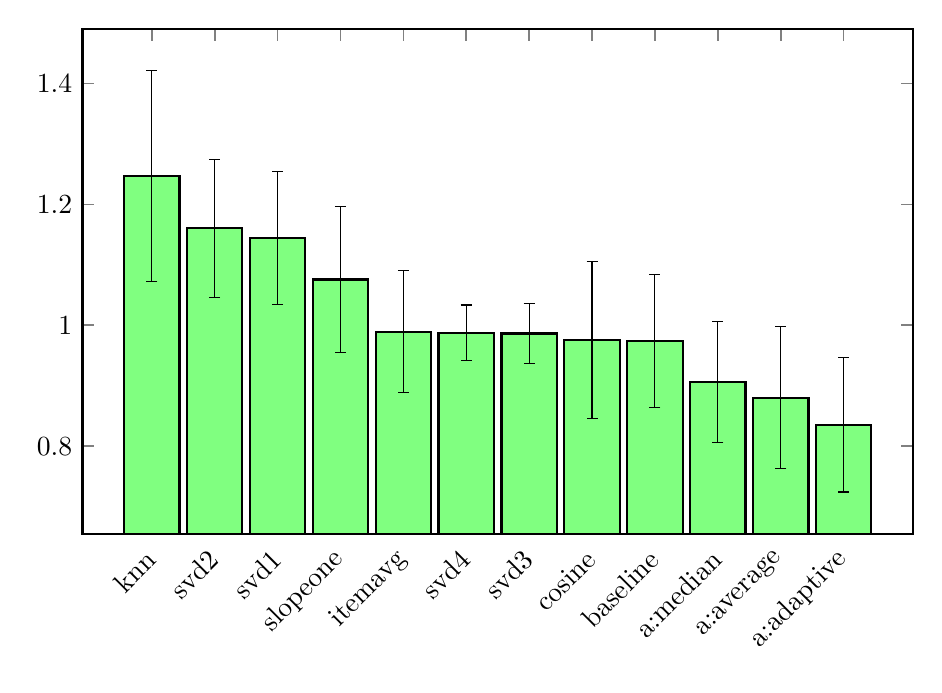
\begin{tikzpicture}

\begin{axis}[
      symbolic x coords={
        knn,svd2,svd1,slopeone,itemavg,svd4,svd3,cosine,baseline,a:median,a:average,a:adaptive},
      xtick=data,
      x tick label style={rotate=45,anchor=east,yshift=-0.5em,xshift=-0.2em},
      bar width=20pt
    ]

    \addplot [ybar,fill=green!50,error bars/.cd,y dir=both,y explicit] coordinates {
      (knn, 1.2467) +- (0,0.17435) 
      (svd2, 1.1605) +- (0,0.11385)
      (svd1, 1.1441) +- (0,0.10985)
      (slopeone, 1.0756) +- (0,0.12075)
      (itemavg, 0.9895) +- (0,0.10115)
      (svd4, 0.9873) +- (0,0.0462)
      (svd3, 0.9865) +- (0,0.04955)
      (cosine, 0.9754) +- (0,0.12975)
      (baseline, 0.9738) +- (0,0.1098)
    %};
    %\addplot [ybar,fill=blue!50] coordinates {
      (a:median, 0.9065) +- (0,0.10025)
      (a:average, 0.8801) +- (0,0.1172)
      (a:adaptive, 0.8352) +- (0,0.11125)
    };
\end{axis}

\end{tikzpicture}
\caption[Average RMSE Plot]{
  Average RMSE plot: This plot shows the average RMSE for each method, and each aggregation method (denoted "a:").
  The actual numbers are given in Table \ref{table:results:e1}.
  The error bars indicate the standard deviation of each method.
  Note the scale on the y-axis --- the errors are not as pronounced as they might seem. 
  See also Figure \ref{plot:datasets}.
}
\label{plot:rmse}
\end{figure}




\begin{figure}[p]
  \centering
  \subfloat[Experiment 1]{\label{fig:rmse:e1}
\pgfplotsset{width=\textwidth,height=8cm}
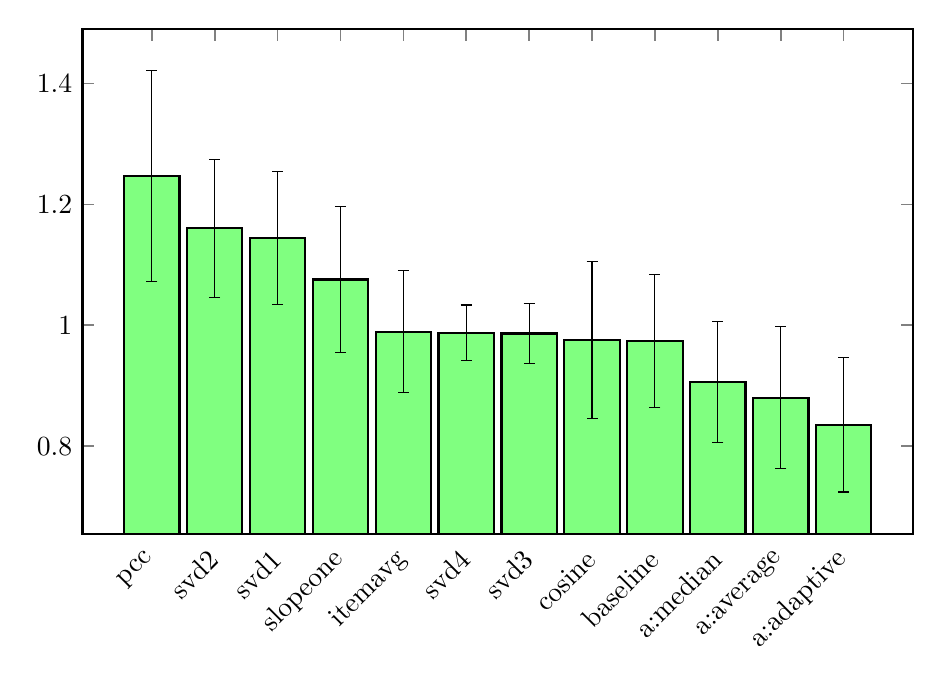
\begin{tikzpicture}
\begin{axis}[
      symbolic x coords={
        pcc,svd2,svd1,slopeone,itemavg,svd4,svd3,cosine,baseline,a:median,a:average,a:adaptive},
      xtick=data,
      x tick label style={rotate=45,anchor=east,yshift=-0.5em,xshift=-0.2em},
      bar width=20pt
    ]
    \addplot [ybar,fill=green!50,error bars/.cd,y dir=both,y explicit] coordinates {
      (pcc, 1.2467) +- (0,0.17435) 
      (svd2, 1.1605) +- (0,0.11385)
      (svd1, 1.1441) +- (0,0.10985)
      (slopeone, 1.0756) +- (0,0.12075)
      (itemavg, 0.9895) +- (0,0.10115)
      (svd4, 0.9873) +- (0,0.0462)
      (svd3, 0.9865) +- (0,0.04955)
      (cosine, 0.9754) +- (0,0.12975)
      (baseline, 0.9738) +- (0,0.1098)
    %};
    %\addplot [ybar,fill=blue!50] coordinates {
      (a:median, 0.9065) +- (0,0.10025)
      (a:average, 0.8801) +- (0,0.1172)
      (a:adaptive, 0.8352) +- (0,0.11125)
    };
\end{axis}
\end{tikzpicture}}

\vspace{1em}
 
  \subfloat[Experiment 2]{\label{fig:rmse:e2}
\pgfplotsset{width=\textwidth,height=8cm}
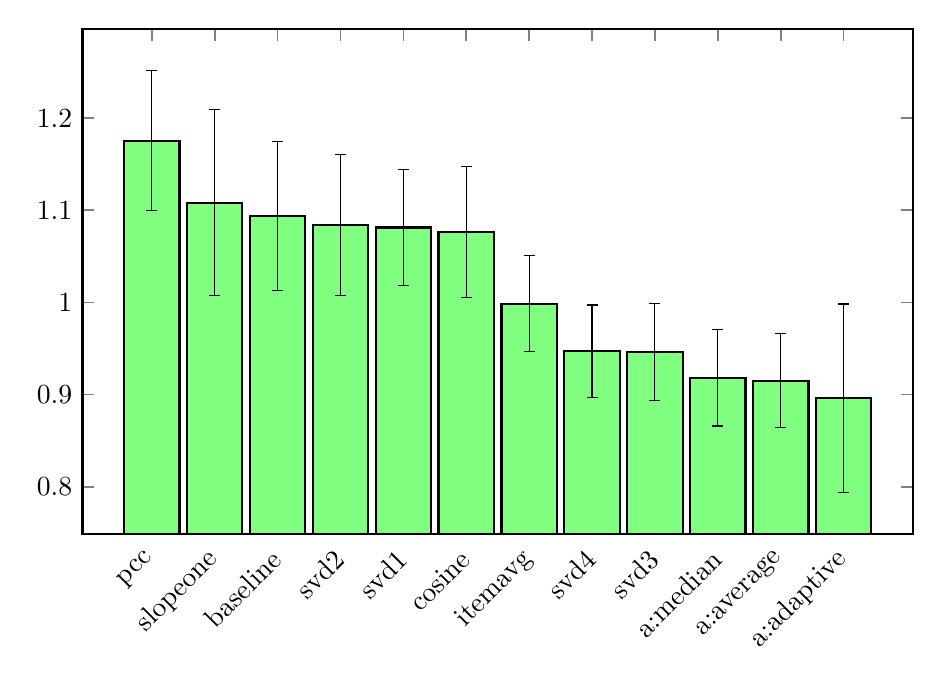
\begin{tikzpicture}
\begin{axis}[
      symbolic x coords={
        pcc,slopeone,baseline,svd2,svd1,cosine,itemavg,svd4,svd3,a:median,a:average,a:adaptive},
      xtick=data,
      x tick label style={rotate=45,anchor=east,yshift=-0.5em,xshift=-0.2em},
      bar width=20pt
    ]
    \addplot [ybar,fill=green!50,error bars/.cd,y dir=both,y explicit] coordinates {
      (pcc, 1.175422) +- (0,0.0758) 
      (slopeone, 1.10813) +- (0,0.101039)
      (baseline, 1.09358) +- (0,0.080985)
      (svd2, 1.084098) +- (0,0.076837)
      (svd1, 1.08128) +- (0,0.063377)
      (cosine, 1.076532) +- (0,0.0709)
      (itemavg, 0.99843) +- (0,0.052021)
      (svd4, 0.947158) +- (0,0.050071)
      (svd3, 0.946024) +- (0,0.052801)
    %};
    %\addplot [ybar,fill=blue!50] coordinates {
      (a:median, 0.918404) +- (0,0.052478)
      (a:average, 0.915036) +- (0,0.051037)
      (a:adaptive, 0.896294) +- (0,0.102056)
    };
\end{axis}
\end{tikzpicture}}

\vspace{1em}

  \caption[Plots of Results for Experiments 1 \emph{\&} 2]{
    Plots of the average RMSEs for Experiments 1 \emph{\&} 2.
    The actual numbers are given in Tables \ref{table:results:e1}
    \emph{\&} \ref{table:results:e2}.
    Note the scale on the y-axis --- the errors are not as pronounced as they might seem. 
  }
  \label{plot:rmse}
\end{figure}




\begin{figure}
\center

\pgfplotsset{width=\textwidth,height=8cm}
\pgfplotsset{every axis/.append style={
thick,
tick style={semithick}}}

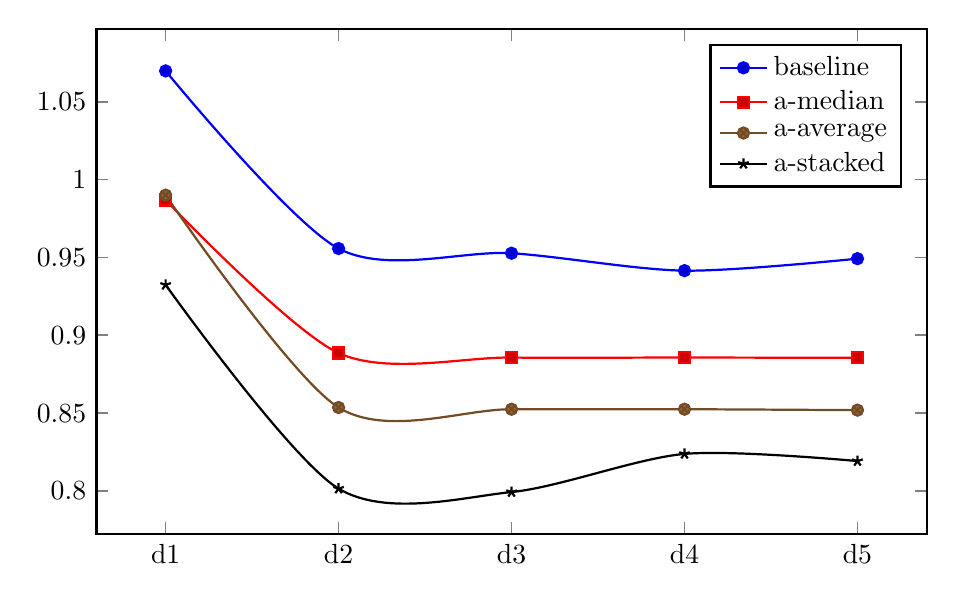
\begin{tikzpicture}

\begin{axis}[
  smooth,
  stack plots=false,
  enlarge x limits=true,
  symbolic x coords={d1,d2,d3,d4,d5},
  xtick=data,
  legend style={
    cells={anchor=west},
    legend pos=north east,
  }
]

\addplot coordinates {
(d1, 1.0698)
(d2, 0.9557)
(d3, 0.9527)
(d4, 0.9415)
(d5, 0.9492)
};
\addlegendentry{baseline}


\addplot coordinates {
(d1, 0.9869)
(d2, 0.8886)
(d3, 0.8857)
(d4, 0.8857)
(d5, 0.8855)
};
\addlegendentry{a-median}
 
\addplot coordinates {
(d1, 0.9900)
(d2, 0.8536)
(d3, 0.8525)
(d4, 0.8525)
(d5, 0.8519)
};
\addlegendentry{a-average}
 
\addplot coordinates {
(d1, 0.9324)
(d2, 0.8015)
(d3, 0.7993)
(d4, 0.8238)
(d5, 0.8192)
};
\addlegendentry{a-stacked}

\end{axis}
\end{tikzpicture}

\caption[RMSE Variations]{
  RMSE Variations: This plot shows that, while the standard deviation of each method may be high,
  this has more to do with the selected dataset than with their performance in comparison with each other.
  The performance of each of the aggregate methods, as well as the best performing standard method,
  follow similar performance paths across the disjoint datasets.
}
\label{plot:datasets}
\end{figure}






Let us take a look at the standard deviation measures from the different methods.
As seen in Figure \ref{plot:rmse}, 
most of the methods, including the stacked models,
exhibit quite a lot of variation in their results.
If these variations occured as a result of unstable
predictions of the same dataset, this would be a substantial problem,
resulting in unreliable predictions.
However, as seen in Figure \ref{plot:datasets},
the standard deviation is mostly caused by the differing
performance across the varying datasets.
As we see, the performance of each of the aggregation methods,
as well as the best performing standard recommender,
follow each other closely. At the same time,
performance varies across the different datasets,
which results in high values for $\sigma$.

What does this mean for hypotheses H1 and H2?
Expressed in terms of this experiment,
H1 posits that stacked recommenders should outperform each of the standard modeling methods
in Table \ref{table:results:e1}.
The adaptive methods blend the results of multiple predictors by estimating the accuracy
on a per-item and per-user basis, satisfying the formulation of H1.

By outperform we mean that our model should have a lower
mean RMSE score than the other singular methods. As we can see in Table \ref{table:results:e1:sum},
\emph{H1 is confirmed for these methods and this dataset}.
While we can not generalize too much on this basis, 
the fact that this dataset is a common testing ground for recommender systems,
that RMSE is the de facto measure for determining performance,
and because of our 5-fold cross-validation, the results allow us 
to confirm hypothesis H1 in these conditions, and likely for other, similar scenarios.
We shall discuss this in Chapter \ref{chap:discussion}.

Similarly, expressed in the same terms, H2 posits that 
our stacked recommenders should outperform the aggregation approaches
given in Table \ref{table:results:e1}.
The \emph{median} and \emph{average} aggregation methods
serve as globalized and generalized aggragation methods,
Stacked recommenders are adaptive in that each prediction is 
aggregated based on the current user and item,
satisfying the language of H2.

As we can see in Table \ref{table:results:e1:sum},
\emph{H2 is confirmed for these methods and this dataset}.
However, as our collection of aggregation methods is a lot simpler
than our collection of recommender systems, the strength of this combination
is notably weaker than that of H1.
Still, the fact that a stacked recommender outperforms these simple aggregation
approaches is a positive result warranting further experiments.
This will also be discussed in Chapter \ref{chap:discussion}.

It would seem then that, based on our experiments, available data
and assumptions of evaluation measures, both H1 and H2 are confirmed.
Our adaptive aggregation approach outperforms both standard recommender
methods and simple generalized aggregation methods.
Notably, our approach is more complex than the methods it outperforms,
so the question whether the methods performance is worth its extra complexity becomes important.
We shall discuss this, and other implications of these results in the next chapter.
For now, let us proceed to the second experiment and hypothesis H3.

\clearpage
